% https://github.com/martinhelso/MathDept


\documentclass[UKenglish,8pt,aspectratio=1610]{beamer}

\usepackage[
backend=biber,        % compilateur par défaut pour biblatex
sorting=none,          % trier par nom, année, titre
citestyle=numeric, % style de citation auteur-année
bibstyle=numeric,  % style de bibliographie alphabétique
]{biblatex}
\addbibresource{biblio.bib}

\usetheme[NoLogo]{MathDept}

\usepackage{nicematrix}
\usepackage{varwidth}
\usepackage[utf8]{inputenx} % For æ, ø, å
\usepackage{babel}          % Automatic translations
\usepackage{csquotes}       % Quotation marks
\usepackage{microtype}      % Improved typography
\usepackage{amssymb}        % Mathematical symbols
\usepackage{mathtools}      % Mathematical symbols
\usepackage[absolute, overlay]{textpos} % Arbitrary placement
\setlength{\TPHorizModule}{\paperwidth} % Textpos units
\setlength{\TPVertModule}{\paperheight} % Textpos units
\usepackage{tikz}
\usetikzlibrary{overlay-beamer-styles}  % Overlay effects for TikZ
\usepackage{dsfont}
\usepackage{fontawesome5}
\author{Thomas Aussaguès}
\title{Mandatory exercise 2}
\subtitle{High resolution beamforming on farfield monochromatic signals, \textcolor{red}{MATLAB version}}
\usepackage{siunitx}
\usepackage{graphics}
\graphicspath{{../images/}}	
\usepackage{pgfplots}
\DeclareUnicodeCharacter{2212}{−}
\usepgfplotslibrary{groupplots,dateplot}
\usetikzlibrary{patterns,shapes.arrows}
\pgfplotsset{compat=newest}
\usepackage{color}
\usepackage{colortbl}
\definecolor{darkred}{rgb}{0.6,0.0,0.0}
\definecolor{darkgreen}{rgb}{0,0.50,0}
\definecolor{lightblue}{rgb}{0.0,0.42,0.91}
\definecolor{orange}{rgb}{0.99,0.48,0.13}
\definecolor{grass}{rgb}{0.18,0.80,0.18}
\definecolor{pink}{rgb}{0.97,0.15,0.45}

% listings
\usepackage{listings}

% Python style for highlighting

\usepackage{ulem}
\begin{document}
	
	
	
	
	% General Setting of listings
	\lstset{
		aboveskip=1em,
		breaklines=true,
		abovecaptionskip=-6pt,
		aboveskip=0pt,
		belowskip=0pt,
		captionpos=b,
		escapeinside={\%*}{*)},
		frame=single
	}
	% 0. Basic Color Theme
	\lstdefinestyle{colored}{ %
		basicstyle=\ttfamily,
		backgroundcolor=\color{gray},
		commentstyle=\color{green}\itshape,
		keywordstyle=\color{blue}\bfseries\itshape,
		stringstyle=\color{red},
	}
	% 1. General Python Keywords List
	\lstdefinelanguage{PythonPlus}[]{Python}{
		morekeywords=[1]{,as,assert,nonlocal,with,yield,self,True,False,None,} % Python builtin
		morekeywords=[2]{,__init__,__add__,__mul__,__div__,__sub__,__call__,__getitem__,__setitem__,__eq__,__ne__,__nonzero__,__rmul__,__radd__,__repr__,__str__,__get__,__truediv__,__pow__,__name__,__future__,__all__,}, % magic methods
		morekeywords=[3]{,object,type,isinstance,copy,deepcopy,zip,enumerate,reversed,list,set,len,dict,tuple,range,xrange,append,execfile,real,imag,reduce,str,repr,}, % common functions
		morekeywords=[4]{,Exception,NameError,IndexError,SyntaxError,TypeError,ValueError,OverflowError,ZeroDivisionError,}, % errors
		morekeywords=[5]{,ode,fsolve,sqrt,exp,sin,cos,arctan,arctan2,arccos,pi, array,norm,solve,dot,arange,isscalar,max,sum,flatten,shape,reshape,find,any,all,plot,linspace,legend,quad,polyval,polyfit,hstack,concatenate,vstack,column_stack,empty,zeros,ones,rand,vander,grid,pcolor,eig,eigs,eigvals,svd,qr,tan,det,logspace,roll,min,mean,cumsum,cumprod,diff,vectorize,lstsq,cla,eye,xlabel,ylabel,squeeze,correlate,argmax,abs,np.}, % numpy / math
	}
	% 2. New Language based on Python
	\lstdefinelanguage{PyBrIM}[]{PythonPlus}{
		emph={d,E,a,Fc28,Fy,Fu,D,des,supplier,Material,Rectangle,PyElmt},
	}
	% 3. Extended theme
	\lstdefinestyle{colorEX}{
		basicstyle=\footnotesize,
		backgroundcolor=\color{gray!10},
		commentstyle=\color{darkgreen}\slshape,
		keywordstyle=\color{blue}\bfseries\itshape,
		keywordstyle=[2]\color{blue}\bfseries,
		keywordstyle=[3]\color{grass},
		keywordstyle=[4]\color{red},
		keywordstyle=[5]\color{orange}\bfseries,
		stringstyle=\color{darkred},
		emphstyle=\color{pink}\underbar,
	}
	
	
	\begin{frame}{Table of contents}
		\tableofcontents
	\end{frame}
	\renewcommand{\arraystretch}{1.3}	
	\section{Problem statement}
	\begin{frame}
		\frametitle{Problem statement \cite{twoDecades}}
			\begin{columns}
			\begin{column}{0.574\textwidth}
				\textbf{Geometry}:
				\begin{itemize}
					\item We consider $N_s=2$ monochromatic farfield sources  
					\item We use a linear array with $M=10$ isotropic sensors with element distance $d=0.5\lambda$ and $\lambda=1~\si{\meter}$
					\item We recorded $N=100$ time samples with sampling frequency $\dfrac{1}{T}$
				\end{itemize}
			\textbf{Signal model: }
				\begin{itemize}
					\item  Phase matrix: $\mathbf{A}=\begin{pmatrix}
						1&1\\
						\vdots&\vdots\\
						e^{-jMkd\sin\theta_1}&e^{-jMkd\sin\theta_2}
					\end{pmatrix}\in\mathbb{C}^{M\times 2}$
				\end{itemize}
			\end{column}
			\begin{column}{0.4\textwidth}
				\vspace{-25pt}
				\begin{figure}[h!]
				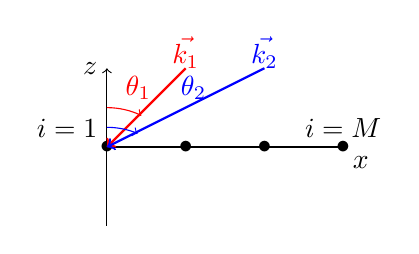
\begin{tikzpicture}
					\draw (1,0)--(4,0);
					\draw (4,0) node [below right] {$x$};
					\draw (1,0) node [above left] {$i=1$};
					\draw (4,0) node [above] {$i=M$};
					\draw [->](1,-1)--(1,1);
					\draw (1,1) node [ left] {$z$};
					
					\foreach \i in {1,...,4}{
						\draw (\i,0) node {$\bullet$};
					}
					
					\draw [<-,red,thick] (1,0)--(2,1);
					\draw[red](2,1.2) node {$\vec{k_1}$};
					
					\draw [<-,blue,thick] (1,0)--(3,1);
					\draw [blue](3,1.2) node {$\vec{k_2}$};
					
					\draw[red, ->] (1,0.5) arc (90:64:1);
					\draw (1.4,0.75) node {\textcolor{red}{$\theta_1$}};
					
					\draw[blue, ->] (1,0.25) arc (90:67:1);
					\draw (2.1,0.75) node {\textcolor{blue}{$\theta_2$}};
					
				\end{tikzpicture}
				\centering
				\caption{Linear array geometry}
			\end{figure}
			\end{column}
		\end{columns} 
\begin{itemize}
	\item  Signal matrix: $\mathbf{S}(t)=\begin{pmatrix}
		a_1e^{j2\pi\Phi_{11}}&\dots&a_1e^{j2\pi\Phi_{1N}}e^{jN\omega_1T}\\
			a_1e^{j2\pi\Phi_{21}}&\dots&a_2e^{j2\pi\Phi_{2N}}e^{jN\omega_2T}
	\end{pmatrix}\in\mathbb{C}^{2\times N}$  where $\Phi_1$ and $\Phi_2$ are two Gaussian random vectors ($\mathcal{N}(0,1)$)
\item Noise vector: $\mathbf{N}(t)$, we assume AWGN
\item Received signal vector: $\mathbf{Y}(t)$
		\begin{equation}
			\mathbf{Y}(t)=\mathbf{A}\mathbf{S}(t) + \mathbf{N}(t)
		\end{equation}
\item Weights vector\footnote{Why is there an $^H$ ? To be coherent with the the output signal calculation: $z(t) =\langle\mathbf{w}\rvert \mathbf{Y}(t)\rangle=\sum_{i=1}^{M}w_iy_i(t)$}: $\mathbf{w}=\begin{pmatrix}
w_1\dots w_M
\end{pmatrix}^H$
\item Steering vector: $\mathbf{a(\theta)}=\begin{pmatrix}
	1&\dots&e^{-jMkd\sin\theta}
\end{pmatrix}^H$
	\end{itemize}
	\end{frame}
	\section{Incoherent sources}
	\subsection{Spatial correlation matrix}
	\begin{frame}
		\frametitle{Spatial correlation matrix estimation  \cite{twoDecades,uncini,Johnson1993ArraySP}}
		\begin{itemize}
			\item In this first part, we consider incoherent sources: $\omega_1\neq\omega_2$ 
			\item One of beamforming challenges is to \textbf{estimate} the spatial correlation matrix $\mathbf{R}=\mathbb{E}\lbrace \mathbf{Y}\mathbf{Y}^H\rbrace$ where $r_{ij}=\mathbb{E}\lbrace y_i(t)y_j(t)^\ast\rbrace$
			\item What estimator should we use? First, we will use $\boldsymbol{\hat{\mathbf{R}}}=\dfrac{1}{N}\mathbf{Y}\mathbf{Y}^H$ (note that we assume W.S.S and ergodicity)
			\item Let's check some properties of $\boldsymbol{\hat{\mathbf{R}}}$
			\item $\boldsymbol{\hat{\mathbf{R}}}$ amplitude is symmetric, its phase is anti-symmetric $\implies\boldsymbol{\hat{\mathbf{R}}}$ is \textbf{hermitian} : $\boldsymbol{\hat{\mathbf{R}}}=\boldsymbol{\hat{\mathbf{R}}}^H$ 
		\end{itemize}
	\vspace{-15pt}
	\begin{columns}
		\begin{column}{0.5\textwidth}
			\begin{figure}[h!]
				\centering
				\includegraphics[scale=0.37]{question1/part_A_question_1_autocorrelation_matrix_amplitude.pdf}
				\caption{Spatial correlation matrix amplitude estimate $\rvert \boldsymbol{\hat{\mathbf{R}}}\rvert$, incoherent signals}
			\end{figure}
		\end{column}
		\begin{column}{0.5\textwidth}
	\begin{figure}[h!]
	\centering
	\includegraphics[scale=0.37]{question1/part_A_question_1_autocorrelation_matrix_phase.pdf}
	\caption{Spatial correlation matrix phase estimate $\arg \boldsymbol{\hat{\mathbf{R}}}$, incoherent signals}
\end{figure}
		\end{column}
	\end{columns} 
\vspace{-10pt}
	\begin{itemize}
	\item Reduced correlation outside the diagonal (brighter colours\footnote{Using Fabio \textsc{CRAMERI's} colormaps \cite{fabio}}): incoherent signals
\end{itemize}
	\end{frame}
	
	\subsection{Standard DAS beamforming}
	\begin{frame}
		\frametitle{DAS power estimate \cite{twoDecades,uncini,Johnson1993ArraySP}}
		\begin{itemize}
			\item For slides 4 to 10, we use the following spatial correlation matrix estimate: $\boldsymbol{\hat{\mathbf{R}}}=\dfrac{1}{N}\mathbf{Y}\mathbf{Y}^H$
			\item Through DAS beamforming, we can get the 'easiest' power estimate
	\begin{equation}
		P(\mathbf{a(\theta)})_{DAS}=\mathbf{a(\theta)}^H\mathbf{R}\mathbf{a(\theta)}
	\end{equation}
\item Is this a 'good' estimate? $\longleftrightarrow$ Is $P(\mathbf{a(\theta)})_{DAS}$ \textbf{unbiased}, \textbf{consistent}\footnote{To estimate the variance, we need to run this experiment several times}?
		\end{itemize}
	
	\begin{columns}
		\begin{column}{0.5\textwidth}
			\begin{figure}[h!]
				\centering
				\includegraphics[scale=0.4]{question2/part_A_question_2_classical_spectrum_estimate.pdf}
				\caption{Classical DAS beamforming power estimate, incoherent signal}
			\end{figure}
		\end{column}
		\begin{column}{0.5\textwidth}
		\begin{itemize}
			\item Obviously, DAS beamforming is not a good choice here! 
			\item The constructed array is unable to distinguish the two signals sources\dots The ideal spectrum should be two \textsc{DIRACs} @ $0~\si{\degree}$ and $-10\si{\degree}$
			\item The two sources are merged into one source
			\item Some side lobes (level $\approx-6~\si{\decibel)}$ around the (large) main lobe
			\item It only requires two matrix multiplication (complexity $\mathcal{O}(N^{2.4})$)
			\item Can we do better?
		\end{itemize}
		\end{column}
	\end{columns}
	\end{frame}

	\subsection{\textsc{CAPON's}/minimum-variance beamformer}
	\begin{frame}
		\frametitle{\textsc{CAPON's}/minimum-variance beamformer \cite{twoDecades,uncini,Johnson1993ArraySP}}
		\begin{itemize}
			\item Adaptive beamforming: let the weights be a function of the incoming signal 
			\item Idea: minimizing the noise power while conserving a unity gain in the steering direction
		\end{itemize}
	\begin{align*}
		\left\{ \begin{aligned}
			&\min P_{MV}(\mathbf{w})=\mathbf{w}^H\mathbf{R}\mathbf{w}\\
			&\text{s.t}~\mathbf{w}^H\mathbf{a(\theta)}=1
		\end{aligned}\right.\implies
		\mathbf{w}=\dfrac{\mathbf{a(\theta)}^H\mathbf{R}^{-1}}{\mathbf{a(\theta)}^H\mathbf{R}^{-1}\mathbf{a(\theta)}}
	~\text{and}~P_{MV}(\mathbf{a(\theta)})=\dfrac{1}{\mathbf{a(\theta)}^H\mathbf{R}^{-1}\mathbf{a(\theta)}}
	\end{align*}
\begin{itemize}
	\item This constrained optimization problem has a closed solution! Which requires a matrix inversion\dots
\end{itemize}
	\begin{columns}
	\begin{column}{0.5\textwidth}
		\begin{figure}[h!]
			\vspace{-15pt}
			\centering
			\includegraphics[scale=0.4]{question3/part_A_question_3_minimum_variance_spectrum_estimate.pdf}
			\caption{Minimum variance power estimate, incoherent signal}
		\end{figure}
	\end{column}
	\begin{column}{0.5\textwidth}
		\begin{itemize}
			\item Some improvements: we have two distinguishable peaks @ $0~\si{\degree}$ and $-10\si{\degree}$
			\item Lower side lobes levels
			\item Lower ML widths
			\item Lower side lobes
			\item The beamformer can distinguish the two signals
			\item But only $10~\si{\decibel}$ between the peaks and the noise level
			\item Inverting a matrix is costly (Complexity: $\mathcal{O}(N^3)$)!
			\item Here, matrix inversion and two matrix multiplication
			\item Can we do better?
		\end{itemize}
	\end{column}
\end{columns}
	\end{frame}
	\subsection{MUSIC method}
	\begin{frame}
		\frametitle{Eigenvalues distribution \cite{twoDecades,uncini,Johnson1993ArraySP}}
		\begin{itemize}
			\item Main idea: 'Find a new base such that $\mathbf{R}$ is a diagonal matrix, get rid of some data and compute its inverse. Then, go back to the standard base.'
			\item $\mathbf{R}$ being \textbf{hermitian} and \textbf{positive semi-definite}, it is diagonalizable and it has a positive spectrum $\text{Sp}(\mathbf{R})\subset\mathbb{R}^{+}$
			\begin{equation}
				\mathbf{R}=\mathbf{V}^H\boldsymbol{\Lambda}\mathbf{V} = \textcolor{blue}{\underbrace{\mathbf{V_s}^H\boldsymbol{\Lambda_s}\mathbf{V_s}}_{\text{signal + noise}} }+ \textcolor{red}{\underbrace{\mathbf{V_n}^H\boldsymbol{\Lambda_n}\mathbf{V_n}}_{\text{noise}}}
		\end{equation}
		\end{itemize}
		\begin{columns}
		\begin{column}{0.5\textwidth}
			\begin{figure}[h!]
				\vspace{-15pt}
				\centering
				\includegraphics[scale=0.4]{question4/part_A_question_4_eigenvalues_distribution.pdf}
				\caption{Eigenvalues distribution for two incoherent sources}
			\end{figure}
		\end{column}
		\begin{column}{0.5\textwidth}
			\begin{itemize}
				\item Two eigenvalues are larger than the other ($\lambda_1=26$ and $\lambda_2=20$) : we can identify both the signal+noise and noise only subspaces
				\item Moreover, we get the number of sources $N_s=2$
				\item Same number of sources as in the simulation parameters \textcolor{green}{\faCheck}
				\item Note that if we have \textit{a priori} knowledge about the noise power ($\sigma_n^2$), we can easily estimate the number of sources: $\lambda_{i\leq N_S}>\sigma_n^2=1$ and $\lambda_{i>N_S}=\sigma_n^2=1$
			\end{itemize}
		\end{column}
	\end{columns}
	\end{frame}
\begin{frame}
	\frametitle{MUSIC algorithm \cite{twoDecades,uncini,Johnson1993ArraySP}}
	\begin{itemize}
		\item We estimate the beamformer power output using only the \textbf{normalized} noise part in the previous eigendecomposition
		\begin{equation}
			\mathbf{R}=\mathbf{V}^H\boldsymbol{\Lambda}\mathbf{V} = \textcolor{blue}{\underbrace{\mathbf{V_s}^H\boldsymbol{\Lambda}_{\mathbf{s}}\mathbf{V_s}}_{\text{signal + noise}} }+ \textcolor{red}{\underbrace{\mathbf{V_n}^H\boldsymbol{\Lambda}_{\mathbf{n}}\mathbf{V_n}}_{\text{noise}}}\approx \textcolor{red}{\mathbf{V_n}^H\boldsymbol{\Lambda}_{\mathbf{n}}\mathbf{V_n}}\implies \underbrace{\mathbf{R}^{-1}\approx \mathbf{V_n}\boldsymbol{\Lambda}_{\mathbf{n}}^{-1}\mathbf{V_n}^H\approx\mathbf{V_n}\mathbf{V_n}^H}_{\text{normalized }\boldsymbol{\Lambda}_{\mathbf{n}}^{-1}=I_n}
		\end{equation}
	\item Why is it efficient? $\boldsymbol{\Lambda}$ is a diagonal matrix so its inverse is easy to compute
	\begin{equation}
		P(\mathbf{a(\theta)})_{MUSIC}=\dfrac{1}{\mathbf{a(\theta)}\mathbf{V_n}\mathbf{V_n}^H\mathbf{a(\theta)}^H}
	\end{equation}
	\end{itemize}
\begin{columns}
	\begin{column}{0.5\textwidth}
		\begin{figure}[h!]
			\vspace{-15pt}
			\centering
			\includegraphics[scale=0.4]{question5/part_A_question_5_music_spectrum_estimate.pdf}
			\caption{MUSIC power estimate}
		\end{figure}
	\end{column}
	\begin{column}{0.5\textwidth}
		\begin{itemize}
			\item Thinner $-3~\si{\decibel}$ main lobes widths
			\item Lower ML widths than the MV beamformer!
			\item We can clearly distinguish the two sources$\implies$ DOA estimation \textcolor{green}{\faCheck}
			\item No more side lobes, outside the peaks the spectrum is flat with a mean level of $-25~\si{\decibel}$ \textcolor{green}{\faCheck}
			\item Altough having the same SNR, the two sources do not have the same level in the spectrum
			\item Not a reliable power (level) estimate \textcolor{red}{\faTimes}
		\end{itemize}
	\end{column}
\end{columns}
\end{frame}
	\subsection{Eigenvector method}
	\begin{frame}
	\frametitle{Eigenvector method \cite{twoDecades,uncini,Johnson1993ArraySP}}
	\begin{itemize}
		\item We estimate the beamformer power output using only the \textbf{non-normalized} noise part in the previous eigendecomposition
		\begin{equation}
			\mathbf{R}=\mathbf{V}^H\boldsymbol{\Lambda}\mathbf{V} = \textcolor{blue}{\underbrace{\mathbf{V_s}^H\boldsymbol{\Lambda}_{\mathbf{s}}\mathbf{V_s}}_{\text{signal + noise}} }+ \textcolor{red}{\underbrace{\mathbf{V_n}^H\boldsymbol{\Lambda}_{\mathbf{n}}\mathbf{V_n}}_{\text{noise}}}\approx \textcolor{red}{\mathbf{V_n}^H\boldsymbol{\Lambda}_{\mathbf{n}}\mathbf{V_n}}\implies \mathbf{R}^{-1}\approx \mathbf{V_n}\boldsymbol{\Lambda}_{\mathbf{n}}^{-1}\mathbf{V_n}^H
		\end{equation}
		\item Why is it efficient? $\boldsymbol{\Lambda}$ is a diagonal matrix so its inverse is easy to compute
		\begin{equation}
			P(\mathbf{a(\theta)})_{EV}=\dfrac{1}{\mathbf{a(\theta)}\mathbf{V_n}\boldsymbol{\Lambda}_{\mathbf{n}}^{-1}\mathbf{V_n}^H\mathbf{a(\theta)}^H}
		\end{equation}
	\end{itemize}
	\begin{columns}
		\begin{column}{0.5\textwidth}
			\begin{figure}[h!]
				\vspace{-15pt}
				\centering
				\includegraphics[scale=0.4]{question6/part_A_question_6_eigenvector_spectrum_estimate.pdf}
				\caption{EV method power estimate}
			\end{figure}
		\end{column}
		\begin{column}{0.5\textwidth}
			\begin{itemize}
			\item Both MUSIC and EV power estimates have low ML widths \textcolor{green}{\faCheck}
			\item They suffer from the same problem on power peak level estimation \textcolor{red}{\faTimes}
			\item The MUSIC algorithm gives thinner peaks (@$-10~\si{\decibel}$)
			\item The MUSIC power estimate seems more flat outside the peaks region
			\end{itemize}
		\end{column}
	\end{columns}
	\end{frame}
\begin{frame}
	\frametitle{Incorrect number of sources $N_s$}
	\begin{itemize}
		\item Using MUSIC and EV algorithm provides better results but a the cost of some \textit{a priori} knowledge : \textbf{the number of sources $N_s$ must be known!}
		\item What happens when using an incorrect number of sources? 
	\end{itemize}

	\begin{columns}
	\begin{column}{0.33\textwidth}
	\begin{figure}[h!]
		\vspace{-15pt}
		\centering
		\includegraphics[scale=0.3]{question7/part_A_question_7_number_of_sources_+Ns=0.pdf}
		\caption{MUSIC \& EV power estimates, $N_s=0$}
	\end{figure}
	\end{column}
	\begin{column}{0.33\textwidth}
\begin{figure}[h!]
	\vspace{-15pt}
	\centering
	\includegraphics[scale=0.3]{question7/part_A_question_7_number_of_sources_+Ns=1.pdf}
		\caption{MUSIC \& EV power estimates, $N_s=1$}
\end{figure}
	\end{column}
\begin{column}{0.33\textwidth}
	\begin{figure}[h!]
		\vspace{-15pt}
		\centering
		\includegraphics[scale=0.3]{question7/part_A_question_7_number_of_sources_+Ns=3.pdf}
			\caption{MUSIC \& EV power estimates, $N_s=3$}
	\end{figure}
\end{column}
\end{columns}
\begin{itemize}
	\item Note that for $N_s=0$, the EV power estimate perfectly fits the MV estimate:
	\begin{equation}
	P_{MUSIC}(\mathbf{a(\theta)})=\left(\sum_{i=N_s+1}^{M}\rVert \mathbf{a(\theta)}^H\mathbf{v_i}\rVert^2\right)^{-1}=\left(\sum_{i=1+0}^M\rVert \mathbf{a(\theta)}^H\mathbf{v_i}\rVert^2\right)^{-1}=P_{MV}(\mathbf{a(\theta)})
	\end{equation} 
\item $N_s<2$: we take into account noise and noise + signal subspaces, larger eigenvalues dominate the others
\item $N_s>2$ : we take into account only the noise subspace so we 'respect' the philosophy of eigendecomposition methods 
\item It seems that the EV method is more robust than the MUSIC one for wrong $N_s$ values
\end{itemize}

\end{frame}
\begin{frame}
	\frametitle{Summary}
		\begin{columns}
		\begin{column}{0.5\textwidth}
			\begin{figure}[h!]
				\centering
				\includegraphics[scale=0.4]{question7/part_A_question_7_all.pdf}
				\caption{DAS, MV, MUSIC \& EV power estimates}
			\end{figure}
		\end{column}
		\begin{column}{0.5\textwidth}
		\begin{table}[h!]
			\begin{tabular}{cccc}
				\hline
				Method&Power estimate&Side lobes&DOA\\
				\hline
				\hline
				DAS&\textcolor{red}{\faTimes}&\textcolor{red}{\faTimes}&\textcolor{red}{\faTimes}\\
				MV&\textcolor{green}{\faCheck}&\textcolor{red}{\faTimes}&\textcolor{orange}{$\sim$}\\
				MUSIC&\textcolor{red}{\faTimes}&\textcolor{green}{\faCheck}&\textcolor{green}{\faCheck}\\
				EV&\textcolor{red}{\faTimes}&\textcolor{green}{\faCheck}&\textcolor{green}{\faCheck}\\
				\hline
			\end{tabular}
		\centering
		\caption{Characteristics of beamforming algorithms}
		\end{table}
	\begin{itemize}
		\item We assumed that sources were incoherent $\longleftrightarrow$ anechoic chamber, without reflections $\longleftrightarrow$ \textbf{anechoic signal propagation model}
		\item To make our simulation more realistic, we can use \textbf{coherent} sources
		\item Similar to a multipath propagation environment: \textbf{echoic signal propagation model}
	\end{itemize}
		\end{column}
	\end{columns} 
\end{frame}
	\section{Coherent sources }
	\begin{frame}{Table of contents}
	\tableofcontents[currentsection]
\end{frame}

\subsection{Standard algorithm}
\begin{frame}
	\frametitle{Spatial correlation matrix for coherent sources \cite{twoDecades,uncini,Johnson1993ArraySP}}
\begin{itemize}
	\item Same problem as before but two sources with the same frequencies and phase terms
	\item We also made the angle between the two sources smaller: $\theta_1=0~\si{\degree}$ and $\theta_2=10~\si{\degree}$
\end{itemize}
	\begin{columns}
	\begin{column}{0.5\textwidth}
		\begin{figure}[h!]
			\centering
			\includegraphics[scale=0.45]{question8/matrices/spatial_correlation_matrix_amplitude.pdf}
			\caption{Spatial correlation matrix amplitude estimate $\rvert \boldsymbol{\hat{\mathbf{R}}}\rvert$, coherent signals}
		\end{figure}
	\end{column}
	\begin{column}{0.5\textwidth}
		\begin{figure}[h!]
			\centering
			\includegraphics[scale=0.45]{question8/matrices/spatial_correlation_matrix_phase.pdf}
			\caption{Spatial correlation matrix phase estimate $\arg \boldsymbol{\hat{\mathbf{R}}}$, coherent signals}
		\end{figure}
	\end{column}
\end{columns} 
\end{frame}
\subsection{EV and MUSIC algorithms for correlated sources}
\begin{frame}
	\frametitle{EV and MUSIC algorithms for correlated sources \cite{twoDecades,uncini,Johnson1993ArraySP}}
\begin{itemize}
	\item Let's try both EV and MUSIC algorithm on correlated sources
\end{itemize}
	\begin{columns}
	\begin{column}{0.5\textwidth}
		\begin{figure}[h!]
			\centering
			\includegraphics[scale=0.45]{question8/part_A_question_8_eigenvalues_distribution.pdf}
			\caption{Eigenvalues distribution, coherent sources}
		\end{figure}
	\end{column}
	\begin{column}{0.5\textwidth}
		\begin{figure}[h!]
			\centering
			\includegraphics[scale=0.45]{question8/spectrums/part_A_question_8_all_spectrums_standard_correlation_matrix.pdf}
			\caption{DAS, MV, MUSIC and EV spectrums for coherent sources}
		\end{figure}
	\end{column}
\end{columns}
\begin{itemize}
	\item Only $1$ eigenvalue for the signal + noise subspace $\implies$ wrong number of sources\dots
\end{itemize}
\end{frame}
\subsection{Modified MUSIC algorithm}
\begin{frame}
	\frametitle{How to improve performances}
\begin{itemize}
	\item We can apply some transformations to $\mathbf{R}$ to suppress or reduce the correlation between sources
	\begin{enumerate}
		\item Spatial averaging or smoothing
		\item Forward-backward transformation
		\item Both the previous transformations
	\end{enumerate}
\item Spatial averaging: compute the correlation matrices of all subarrays with size $L$ ($L=5$ here). It reduces the cross-correlation terms but also reduces the number of sensors: smaller aperture$\implies$ poorer resolution (similar to \textsc{WELCH's} periodogram)
\begin{equation}
	\mathbf{R}=\begin{pNiceMatrix}[margin]
	\Block[draw,fill=red!25,rounded-corners]{2-2}{}
		r_{11}&r_{12}&\dots&r_{1M-1}&r_{1M}\\
		r_{12}^\ast&r_{22}&\dots&r_{2M-1}&r_{2M}\\
		\vdots&\vdots&\Block[draw,fill=red!25,rounded-corners]{1-1}{}\ddots&\vdots&\vdots\\
	
r_{1M-1}^\ast&r_{2M-1}^\ast&\dots&\Block[draw,fill=red!25,rounded-corners]{2-2}{}r_{M-1M-1}&r_{M-1M}\\
r_{1M}^\ast&r_{2M}^\ast&\dots&r_{M-1M}^\ast&r_{MM}
	\end{pNiceMatrix}
\implies\mathbf{R_S}=\dfrac{1}{\underbrace{M+L-1}_{=K}}\sum_{i=1}^{K}\mathbf{R_i}~\text{where}~\mathbf{R_i}=\mathbf{Y}\left[i:L\ast i\right]\mathbf{Y}\left[i:L\ast i\right]^H
\end{equation}

	\item Forward-backward: let $\mathbf{J}=\begin{pNiceMatrix}
		0&\dots&1\\
		\vdots&\ddots&\vdots\\
		1&\dots&0
		
	\end{pNiceMatrix}$ be the exchange matrix. Then, the forward-backward spatial correlation matrix is defined as:
\end{itemize}
\begin{equation}
	\mathbf{R_{FB}}=\dfrac{1}{2}\left(\mathbf{R}+\mathbf{J}\mathbf{R}^\ast\mathbf{J}\right)
\end{equation}
\end{frame}


\begin{frame}
	\frametitle{What transformation should we apply to $\mathbf{R}$? \cite{twoDecades,uncini,Johnson1993ArraySP}}
	\vspace{-15pt}
	\begin{columns}
		\begin{column}{0.33\textwidth}
			\begin{figure}[h!]
				\centering
				\includegraphics[scale=0.3]{question8/matrices/spatial_correlation_matrix_amplitude}
				\caption{Standard $\mathbf{R}$}
			\end{figure}
		\end{column}
		\begin{column}{0.33\textwidth}
			\begin{figure}[h!]
				\centering
				\includegraphics[scale=0.3]{question8/matrices/smoothed_spatial_correlation_matrix_amplitude}
				\caption{Smoothed: $\mathbf{R_S}$}
			\end{figure}
		\end{column}
		\begin{column}{0.33\textwidth}
			\begin{figure}[h!]
				\centering
				\includegraphics[scale=0.3]{question8/matrices/forward_backward_spatial_correlation_matrix_amplitude}
				\caption{Forward-backward: $\mathbf{R_{FB}}$}
			\end{figure}
		\end{column}
	\end{columns}
	
	\begin{columns}
		\begin{column}{0.33\textwidth}
			\vspace{-15pt}
			\begin{figure}[h!]
				\centering
				\includegraphics[scale=0.3]{question8/matrices/forward_backward_smoothed_spatial_correlation_matrix_amplitude}
				\caption{FB + smoothed: $\mathbf{R_{FBS}}$}
			\end{figure}
		\end{column}
		\begin{column}{0.33\textwidth}
			\vspace{-15pt}
			\begin{figure}[h!]
				\centering
				\includegraphics[scale=0.3]{question8/matrices/smoothed_forward_backward_spatial_correlation_matrix_amplitude}
				\caption{Smoothed + FB: $\mathbf{R_{SFB}}$}
			\end{figure}
		\end{column}
		\begin{column}{0.33\textwidth}
			\begin{itemize}
				\item Spatial averaging: reduces correlation outside the diagonal but lower number of sensors$\implies$ lower resolution
			\item Lower aperture size
			\item What is the best choice here? 
			\end{itemize}
		\end{column}
	\end{columns}
\end{frame}

\begin{frame}
	\frametitle{What transformation should we apply to $\mathbf{R}$?}
	\vspace{-18pt}
	\begin{columns}
	\begin{column}{0.33\textwidth}
	\begin{figure}[h!]
		\centering
		\includegraphics[scale=0.27]{question8/spectrums/part_A_question_8_all_spectrums_standard_correlation_matrix}
		\caption{Standard $\mathbf{R}$}
	\end{figure}
\end{column}
	\begin{column}{0.33\textwidth}
	\begin{figure}[h!]
		\centering
		\includegraphics[scale=0.27]{question8/spectrums/part_A_question_8_all_spectrums_smoothed_correlation_matrix}
	\caption{Smoothed: $\mathbf{R_S}$}
	\end{figure}
\end{column}
	\begin{column}{0.33\textwidth}
	\begin{figure}[h!]
		\centering
		\includegraphics[scale=0.27]{question8/spectrums/part_A_question_8_all_spectrums_forward_backward_correlation_matrix}
		\caption{Forward-backward: $\mathbf{R_{FB}}$}
	\end{figure}
\end{column}
\end{columns}
\begin{columns}
	\begin{column}{0.33\textwidth}
		\vspace{-15pt}
	\begin{figure}[h!]
		\centering
		\includegraphics[scale=0.27]{question8/spectrums/part_A_question_8_all_spectrums_forward_backward_smoothed_spatial_correlation_matrix}
		\caption{FB + smoothed: $\mathbf{R_{FBS}}$}
	\end{figure}
\end{column}
	\begin{column}{0.33\textwidth}
		\vspace{-15pt}
	\begin{figure}[h!]
		\centering
		\includegraphics[scale=0.27]{question8/spectrums/part_A_question_8_all_spectrums_smoothed_forward_backward_spatial_correlation_matrix}
		\caption{Smoothed + FB: $\mathbf{R_{SFB}}$}
	\end{figure}
\end{column}
	\begin{column}{0.33\textwidth}
\begin{itemize}
	\item FB, FB + smoothed and smoothed FB techniques provide the best results here
	\item Acceptable DOA estimates and ML width
	\item We can not judge the resolution\dots 
	\item To do it, we will to need run the previous experiment for multiple DOA $\theta$ and see what is the smallest angle difference such that two sources can be resolved
\end{itemize}
\end{column}
\end{columns}
\end{frame}



\begin{frame}
	\frametitle{Bias and ML width}
\begin{itemize}
	\item We have seen that using EV/MUSIC algorithms combined with a forward-backward smoothed (or smoothed forward-backward) spatial correlation matrix improved the 'quality' of the power estimate
	\item Since both EV and MUSIC methods have similar results, we focus on assessing MUSIC performances
	\item What is the 'right' choice for the correlation matrix estimate? Let's compare the bias and the ML width
\end{itemize}
\begin{table}
	\begin{tabular}{cccccc}
		\hline
		$\mathbf{R}$ estimate& $\theta_1$ ($\si{\degree}$)&ML width $\Delta\theta_1$ ($\si{\degree}$)&$\theta_2$ ($\si{\degree}$)&ML width $\Delta\theta_2$ ($\si{\degree}$)&Min level ($\si{\decibel}$)\\
		\hline
			\hline
Standard&-14.390&26.770&-0.090&27.600&-3.136\\
Smoothed&-2.850&1.985&7.820&7.925&-25.319\\
FB&-0.120&0.620&9.770&0.650&-23.244\\
FB + smoothed&-1.260&0.310&8.880&0.415&-41.971\\
Smoothed + FB&-1.220&0.375&9.020&0.900&-40.113\\
		\hline
	\end{tabular}
\centering
\caption{DOA estimation, resolution and minimum power level for the MUSIC algorithm}
\end{table}

\begin{columns}
	\begin{column}{0.5\textwidth}
	\begin{table}
		\begin{tabular}{ccc}
			\hline
			$\mathbf{R}$ estimate&Mean error ($\si{\degree}$)&Mean ML width ($\si{\degree}$)\\
			\hline
			\hline
			Standard&\cellcolor{red!25}12.240&\cellcolor{red!25}27.185\\
			Smoothed&\cellcolor{red!25}2.515&\cellcolor{red!25}4.955\\
			FB&\cellcolor{green!25}0.175&\cellcolor{green!25}0.635\\
			FB + smoothed&\cellcolor{orange!25}1.190&\cellcolor{green!25}0.362\\
			Smoothed + FB&\cellcolor{orange!25}1.100&\cellcolor{green!25}0.637\\
			\hline
		\end{tabular}
		\centering
		\caption{Mean DOA estimation error and mean resolution for the MUSIC algorithm}
	\end{table}
	\end{column}
	\begin{column}{0.5\textwidth}
		\begin{itemize}
			\item Standard and smoothed $\mathbf{R}$ estimates provide poor results\dots
			\item According to these tables, FB, FB + smoothed and smoothed + FB correlation matrices give the best results
			\item FB provides an excellent DOA estimation but with a acceptable ML width whereas FB + smoothed and smoothed + FB give an higher bias but better ML width
			\item Trade-off\dots Here, we focus on the FB $\mathbf{R}$ estimate
		\end{itemize}
	\end{column}
\end{columns}

\end{frame}
\begin{frame}
	\frametitle{SNR}
\begin{itemize}
	\item How are performances affected when decreasing the SNR?
\end{itemize}
\begin{columns}
	\begin{column}{0.5\textwidth}
		\begin{figure}[h!]
			\vspace{-15pt}
			\centering
			\includegraphics[scale=0.35]{snr_analysis/DOA_estimation_vs_snr_forward_backward_correlation_matrix.pdf}
			\caption{Estimated DOAs vs. SNR, FB + smoothed}
		\end{figure}
	\end{column}
	\begin{column}{0.5\textwidth}
		\begin{figure}[h!]
		\vspace{-15pt}
		\centering
		\includegraphics[scale=0.35]{snr_analysis/mean_error_and_resolution_vs_snr_forward_backward_correlation_matrix}
		\caption{Mean error and ML width vs. SNR, FB + smoothed}
	\end{figure}
	\end{column}
\end{columns}
\begin{itemize}
	\item Decreasing the SNR leads to poor performances as expected (better to use other methods such as root MUSIC)
	\item Optimal SNR value: $6~\si{\decibel}$
\end{itemize}
\end{frame}
\section{Additional slides}
\begin{frame}
	\frametitle{Stationarity and ergodicity}
\begin{itemize}
	\item We assume that $\mathbf{Y}$ was a W.S.S ergodic stochastic process. Is that really the case?
	\item One way to answer this question is to plot $\mathbf{Y}$ as a 2D-image\footnote{Note that this is only a first order test\dots}
\end{itemize}

\begin{columns}
\begin{column}{0.5\textwidth}
	\begin{figure}[h!]
		\vspace{-15pt}
		\centering
		\includegraphics[scale=0.5]{question1/part_A_question_1_WSS_ergodicity.pdf}
		\caption{$\mathbf{Y}$ amplitude and phase as 2D-images}
	\end{figure}
\end{column}
\begin{column}{0.5\textwidth}
\textbf{Stationarity}
\begin{itemize}
	\item If $\mathbf{Y}$ is an stationary process then its statistical properties are constant with time
	\item So if we look at two vertical cuts of both images at two time instants, then the mean along these cuts should be the same
	\item \textbf{Stationarity} \textcolor{green}{\faCheck}
\end{itemize}
\textbf{Ergodicity}
\begin{itemize}
	\item If $\mathbf{Y}$ is an ergodic process then its time average is equal to its ensemble average
	\item So if we take two horizontal cuts of both images at two time instants, then the mean along these cuts should be the same
	\item \textbf{Ergodicity} \textcolor{green}{\faCheck}
\end{itemize}
\end{column}
\end{columns}

\end{frame}

\begin{frame}
	\frametitle{Diagonal loading and rotary averaging}
\begin{itemize}
	\item Diagonal loading: $\mathbf{R}_{DL}=\mathbf{R}(1-\delta \mathbf{I_M}), \delta\in\mathbb{R}$
	\item Rotary averaging: $\mathbf{R_{RA}}=\dfrac{1}{4}\left(\mathbf{R}+\mathbf{J}\mathbf{R}^T+\mathbf{J}\mathbf{R}+\mathbf{R}\mathbf{J}\right)$
\end{itemize}
\vspace{-10pt}
\begin{columns}

	\begin{column}{0.25\textwidth}
		\begin{figure}[h!]
			\centering
			\includegraphics[height=3cm]{question8/matrices/diagonaly_loaded_spatial_correlation_matrix_amplitude.pdf}
			\caption{$\mathbf{R_{DL}}$ squared magnitude}
		\end{figure}
	\end{column}
	\begin{column}{0.25\textwidth}
	\begin{figure}[h!]
		\centering
		\includegraphics[height=3cm]{question8/matrices/diagonaly_loaded_spatial_correlation_matrix_phase.pdf}
		\caption{$\mathbf{R_{DL}}$ phase}
	\end{figure}
\end{column}
	\begin{column}{0.25\textwidth}
	\begin{figure}[h!]
	\centering
	\includegraphics[height=3cm]{question8/spectrums/part_A_question_8_all_spectrums_diagonaly_loaded.pdf}
	\caption{Power estimates, $\mathbf{R_{DL}}$}
\end{figure}
\end{column}
	\begin{column}{0.25\textwidth}
\begin{itemize}
	\item Does not work\dots
\end{itemize}
\end{column}
\end{columns}
\vspace{-13pt}
\begin{columns}
	\begin{column}{0.25\textwidth}
		\begin{figure}[h!]
			\centering
			\includegraphics[height=3cm]{question8/matrices/rotary_averaged_spatial_correlation_matrix_amplitude.pdf}
			\caption{$\mathbf{R_{RA}}$ squared magnitude}
		\end{figure}
	\end{column}
	\begin{column}{0.25\textwidth}
		\begin{figure}[h!]
			\centering
			\includegraphics[height=3cm]{question8/matrices/rotary_averaged_spatial_correlation_matrix_phase.pdf}
			\caption{$\mathbf{R_{RA}}$ phase}
		\end{figure}
	\end{column}
	\begin{column}{0.25\textwidth}
		\begin{figure}[h!]
			\centering
			\includegraphics[height=3cm]{question8/spectrums/part_A_question_8_all_spectrums_rotary_averaged.pdf}
			\caption{Power estimates, $\mathbf{R_{RA}}$}
		\end{figure}
	\end{column}
	\begin{column}{0.25\textwidth}
		\begin{itemize}
			\item Does not work\dots
		\end{itemize}
	\end{column}
\end{columns}

\end{frame}
\begin{frame}
	\frametitle{References}
	\printbibliography
\end{frame}
%\begin{frame}
	%\begin{itemize}
		%\item Rotary averaging:
		%\item Diagonal reducing:
	%\end{itemize}
%\end{frame}

		
	
\end{document}